\subsection{Hardware Requirements}
\label{sec:hw_req}

%\begin{figure}[t]%
%	\centering
%	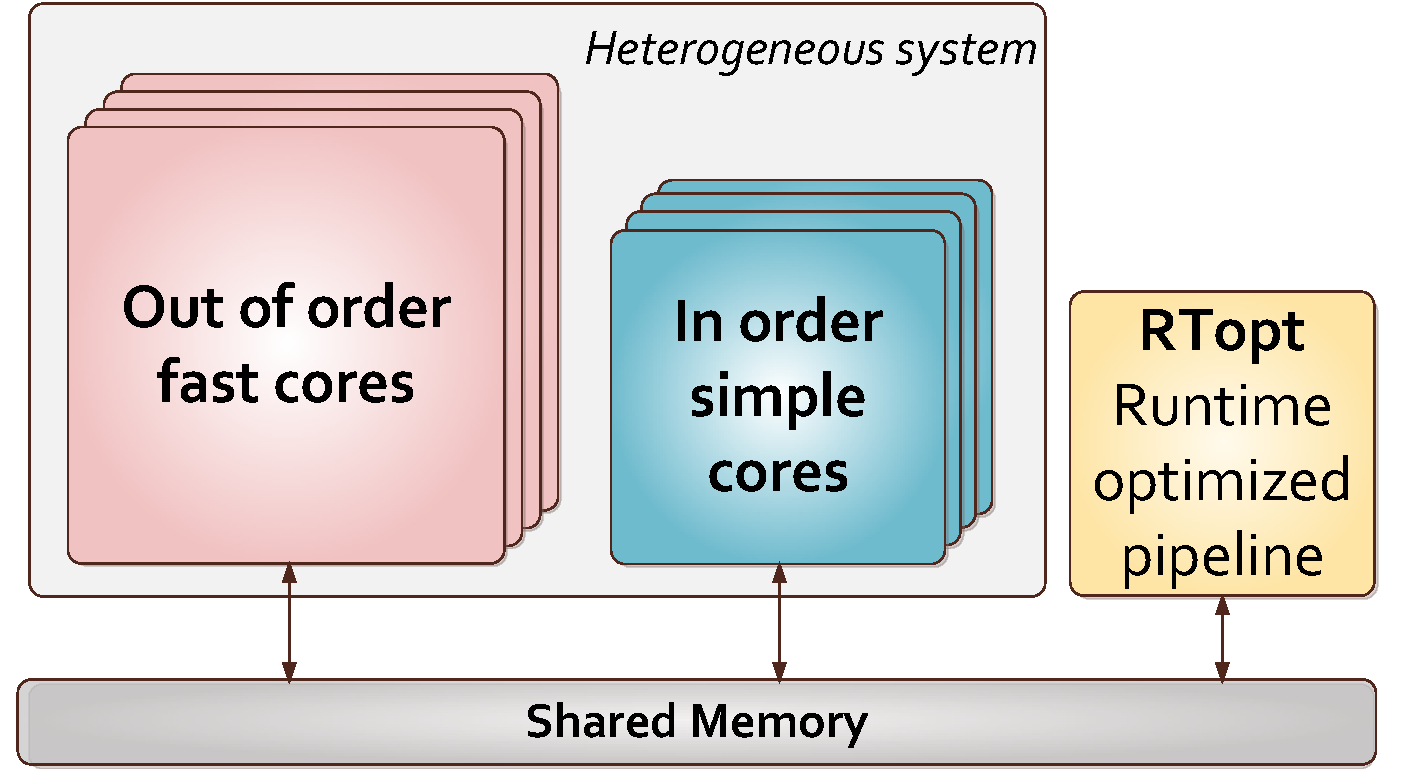
\includegraphics[width=0.6\columnwidth]{figures/hw_fig.pdf}
%	\caption{SoC architecture including three types of cores: out of order, in-order and RTopt.}
%	\label{fig:hw}%
%	\vspace{-0.3cm}
%\end{figure}
As described in the previous section, {\proposal} assumes the existence of specialized hardware that accelerates the task creation step. 
The goal of this paper is not to propose a detailed micro-architecture of the specialized hardware; instead we sketch the high-level hardware requirements for the {\proposal} set-up, in the hope to be an insightful and useful influence for hardware designers.
The SRT is bound to the task creation accelerator and executes the requests in the RRQ. 
Previous studies have proposed custom accelerators for the runtime activity~\cite{TaskSS, Xubin, Nexus, Swarm, TMU, Carbon}. 
These proposals significantly accelerate (up to three orders of magnitude) different bottlenecks of the runtime system\footnote{Section~\ref{sec:related} further describes these proposals.}. 
These special purpose designs can only execute runtime system activity.

\begin{figure}[t!]%
	\centering
	\subfloat[Communication mechanism between master/workers and SRT threads.]{\label{fig:communication}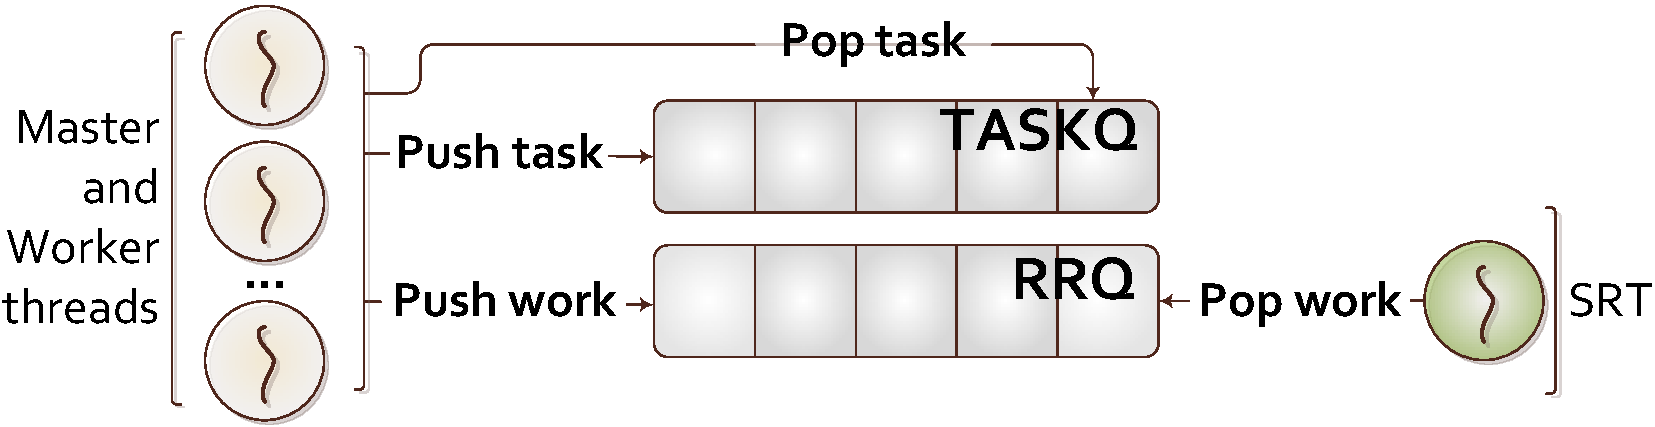
\includegraphics[width=0.5\columnwidth]{figures/communication2.pdf}} \hspace{0.2cm}
	\subfloat[SoC architecture including three types of cores: out of order, in-order and RTopt.]{\label{fig:hw}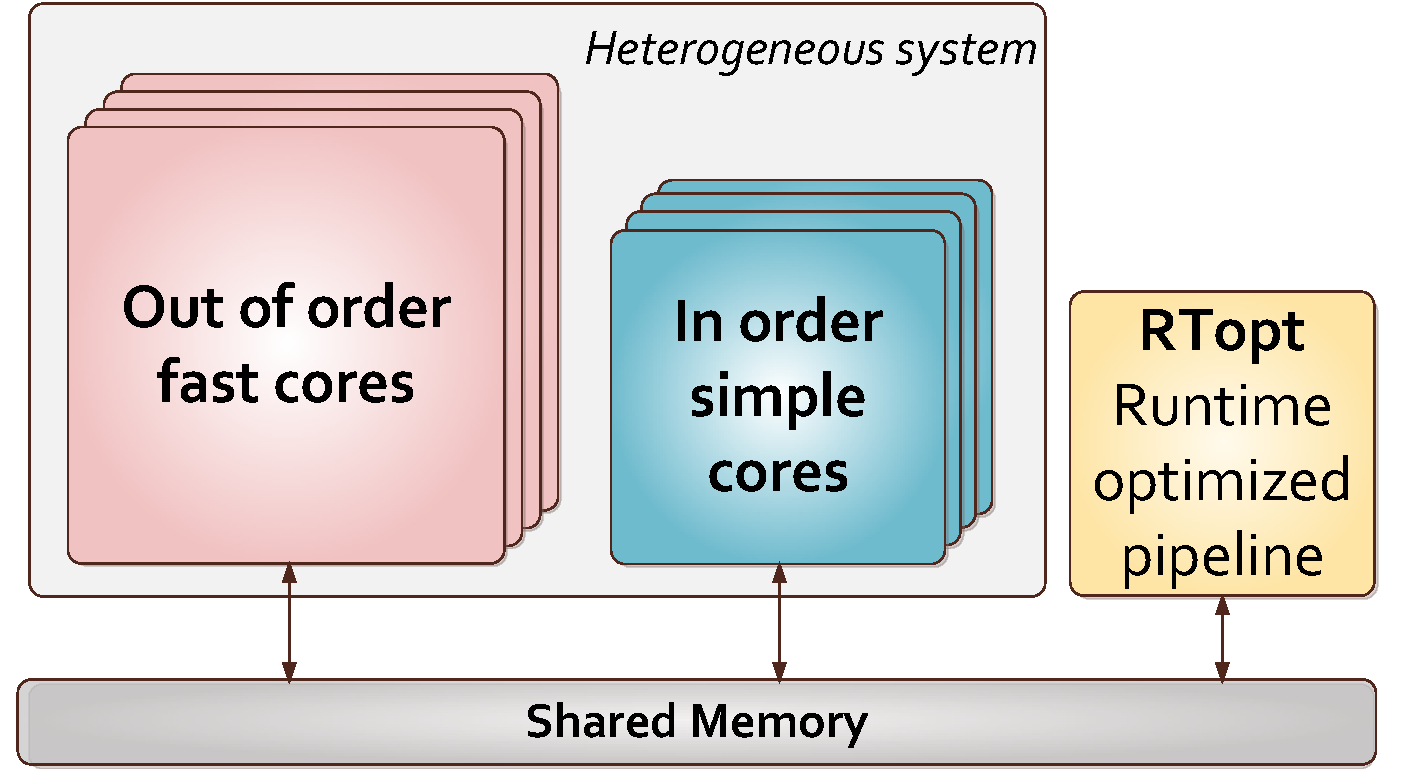
\includegraphics[width=0.4\linewidth]{figures/hw_fig.pdf}}
	\caption{}
\end{figure}


As an alternative, in our envisioned architecture we propose to have a general purpose core that has been optimized to run the runtime system activity more efficiently. 
The runtime optimized (RTopt) core can be combined with both homogeneous or heterogeneous systems and accelerate the runtime activity.
Figure~\ref{fig:hw} shows the envisioned architecture when RTopt is combined with an asymmetric heterogeneous system.
%Figure~\ref{fig:hw} shows the envisioned asymmetric multi-core architecture with different core types. 
This architecture has three core types that consist of simple in-order cores, fast out-of-order cores and an RTopt core for the SRT. 
RTopt can optimize its architecture, having a different cache hierarchy, pipeline configuration and specialized hardware structures to hold and process the SRT. 
As a result, the RTopt executes the SRT much faster than the other cores. 
The RTopt can also execute tasks, but will achieve limited performance compared to the other cores as its hardware structures have been optimized for a specific software (the SRT).

To evaluate our approach we study the requirements of the RTopt in order to provide enough performance for {\proposal}.
Based on the analysis by Etsion et al.~\cite{TaskSS}, there is a certain \textit{task decode rate} that leads to optimal utilization of the multi-core system.
This rule can be applied in the case of {\proposal} for the \textit{task creation rate}, i.e., the frequency of task generation of the runtime system.
If the \textit{task creation rate} is higher than the \textit{task execution rate}, then for a highly parallel application the resources will always have tasks to execute and they will not remain idle.
To achieve a high \textit{task creation rate}, we can accelerate the task creation cost.
Equation~\ref{eq.create} shows the maximum optimal task creation cost, $C_{opt}(x)$ in order to keep $x$ cores busy, without starving due to task creation.

%\begingroup\makeatletter\def\f@size{9}\check@mathfonts
\begin{equation}
  \text{$C_{opt}(x) = avg.\ task\ duration / x$ }
\label{eq.create}
\end{equation}
%\endgroup

If $C_{gp}$ is the cost of task creation when it is performed on a general purpose core, then the RTopt has to achieve a speedup of $r = C_{gp}/C_{opt}(x)$ to achieve full utilization of the system. 
Section~\ref{sec:experimental:simulation} performs an analysis based on these requirements for the evaluated applications. 
As we will see in Section~\ref{sec:experimental:simulation}, a modest and implementable value of $r=16\times$ is enough to significantly accelerate execution on a 512-core system.

Finally, if {\proposal} executes on a regular processor without the RTopt core, the SRT is bound to a regular core without any further modification. In this scenario, applications will not significantly benefit from having a separate SRT.



